\documentclass[12pt, a4]{article}
\usepackage[english]{babel}
\usepackage[utf8x]{inputenc}
\usepackage{fullpage}
\usepackage{listings}
\usepackage{graphicx}
\usepackage{color}

%Syntax highlighting
\definecolor{blue-violet}{rgb}{0.54, 0.17, 0.89}
\definecolor{ao}{rgb}{0.0, 0.5, 0.0}
\definecolor{amaranth}{rgb}{0.9, 0.17, 0.31}
\definecolor{ballblue}{rgb}{0.13, 0.67, 0.8}
\definecolor{onyx}{rgb}{0.06, 0.06, 0.06}


\lstset{
  breaklines=true,                 % automatic line breaking only at whitespace
  captionpos=b,                    % sets the caption-position to bottom
  breakatwhitespace=false,
  keepspaces=true,
  numbers=left,
  numbersep=5pt,
  showspaces=false,
  showstringspaces=false,
  showtabs=false,
  tabsize=4,  
  backgroundcolor=\color{white},   % choose the background color
  commentstyle=\color{ao},    % comment style
  keywordstyle=\color{amaranth},    % keyword style
  stringstyle=\color{blue-violet},    % string literal style
  numberstyle=\tiny\color{ballblue},	   % number style
  basicstyle=\ttfamily\footnotesize\color{onyx} % size of fonts used for the code
}

%Document Header
\title{\textbf{Department of CSE\\SSN College of Engineering}}
\author{\textbf{Vishakan Subramanian - 18 5001 196 - Semester VII}}
\date{20 October 2021}

\begin{document}
\maketitle
\hrule
\section*{\center{UCS 1712 - Graphics And Multimedia Lab}}
\hrule
\bigskip

%Assignment Details
\subsection*{\center{\textbf{Exercise 11: Image Editing and Manipulation}}}
\subsection*{\flushleft{Aim:}}
\begin{flushleft}

\begin{enumerate}

\item Using GIMP, include an image and apply filters, noise and masks.
\item Using GIMP, create a GIF animated image. 

\end{enumerate}
 
\end{flushleft}


%Input
\newpage
\subsection*{\flushleft{Input: Base Image}}
\begin{figure}[h]
\centering
\caption{Base Image.}
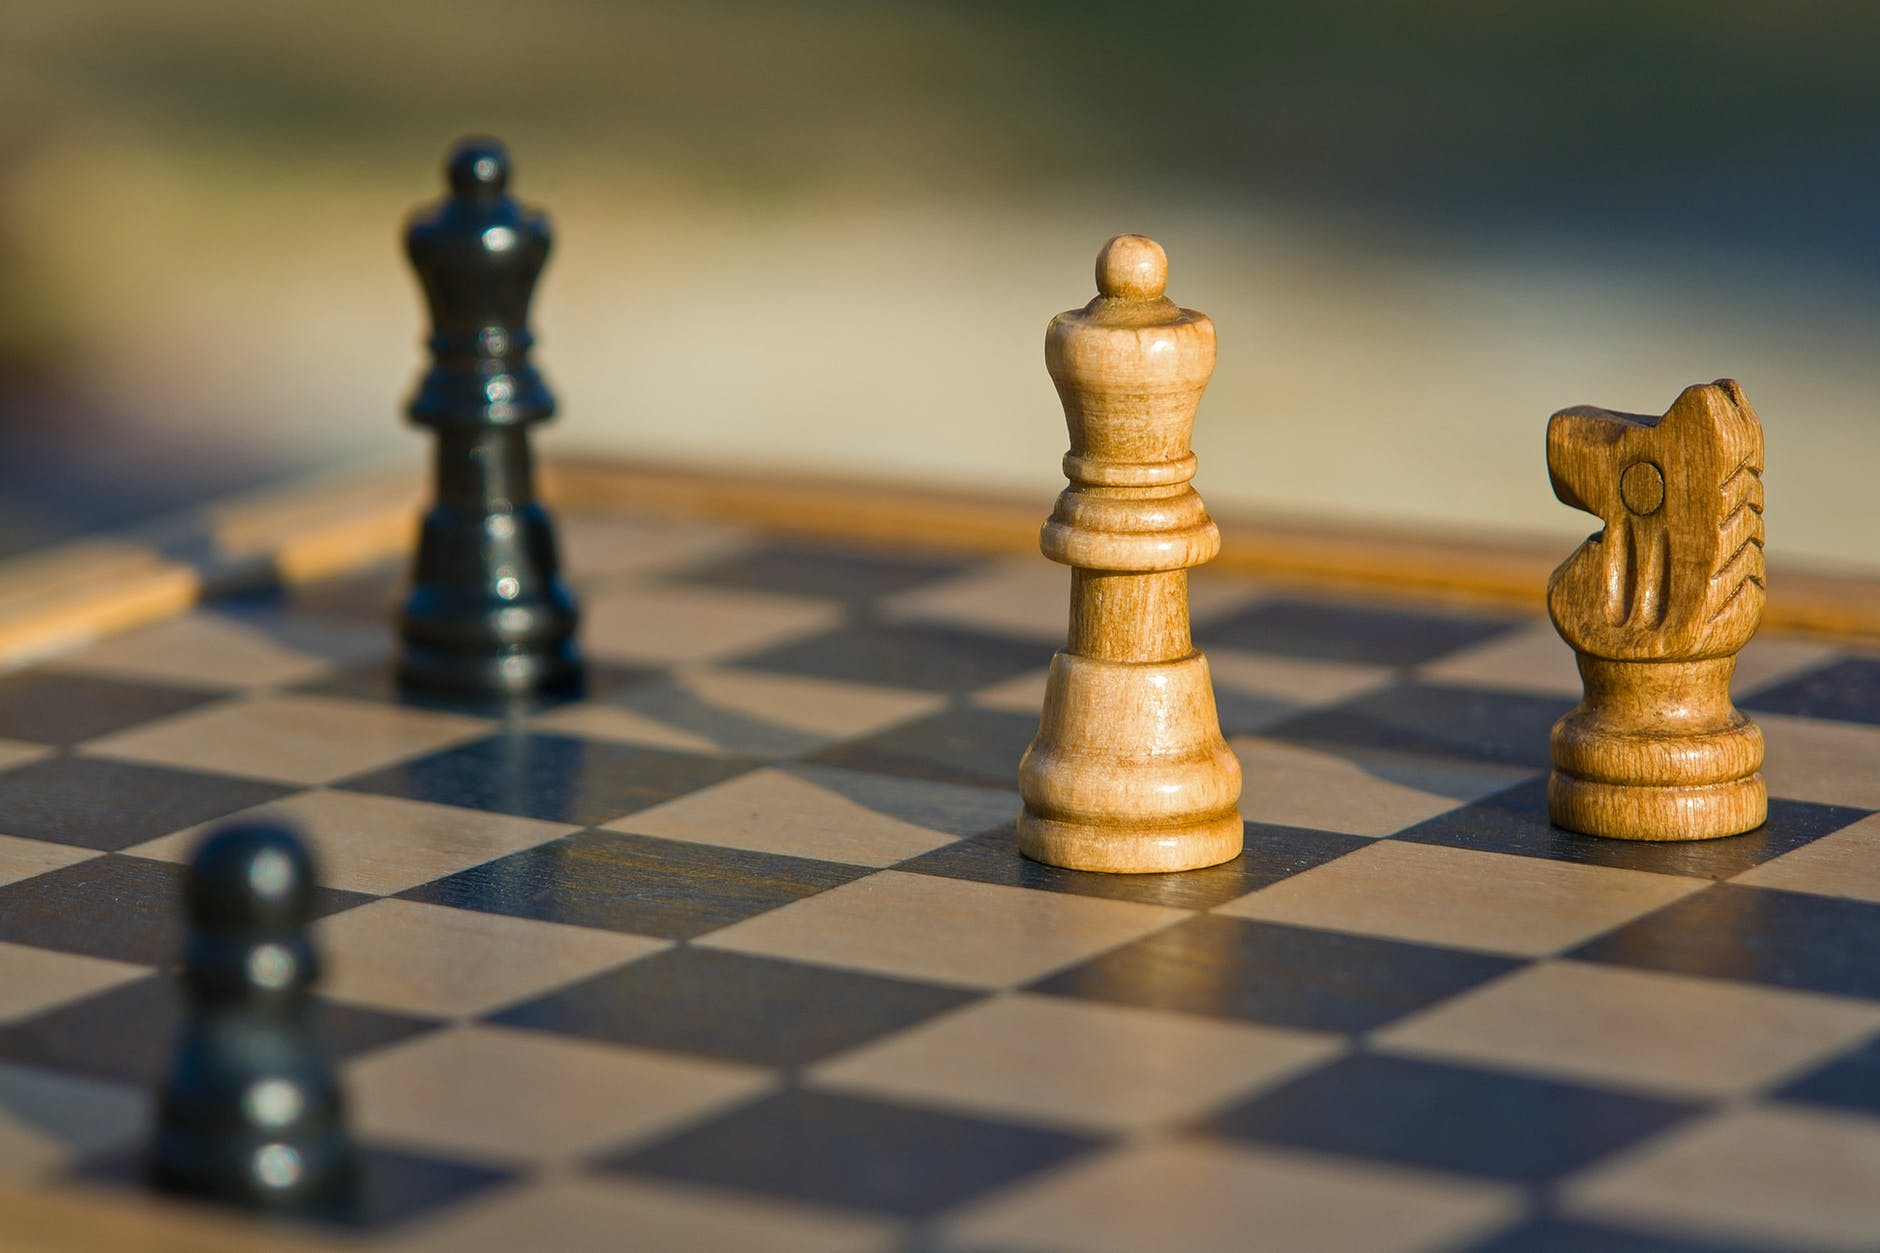
\includegraphics[height=7cm, width=12cm]{Chess.jpeg}
\end{figure}


%Output
\newpage
\subsection*{\flushleft{Output: Filter - Vignette}}
\begin{figure}[h]
\centering
\caption{Filter: Vignette}
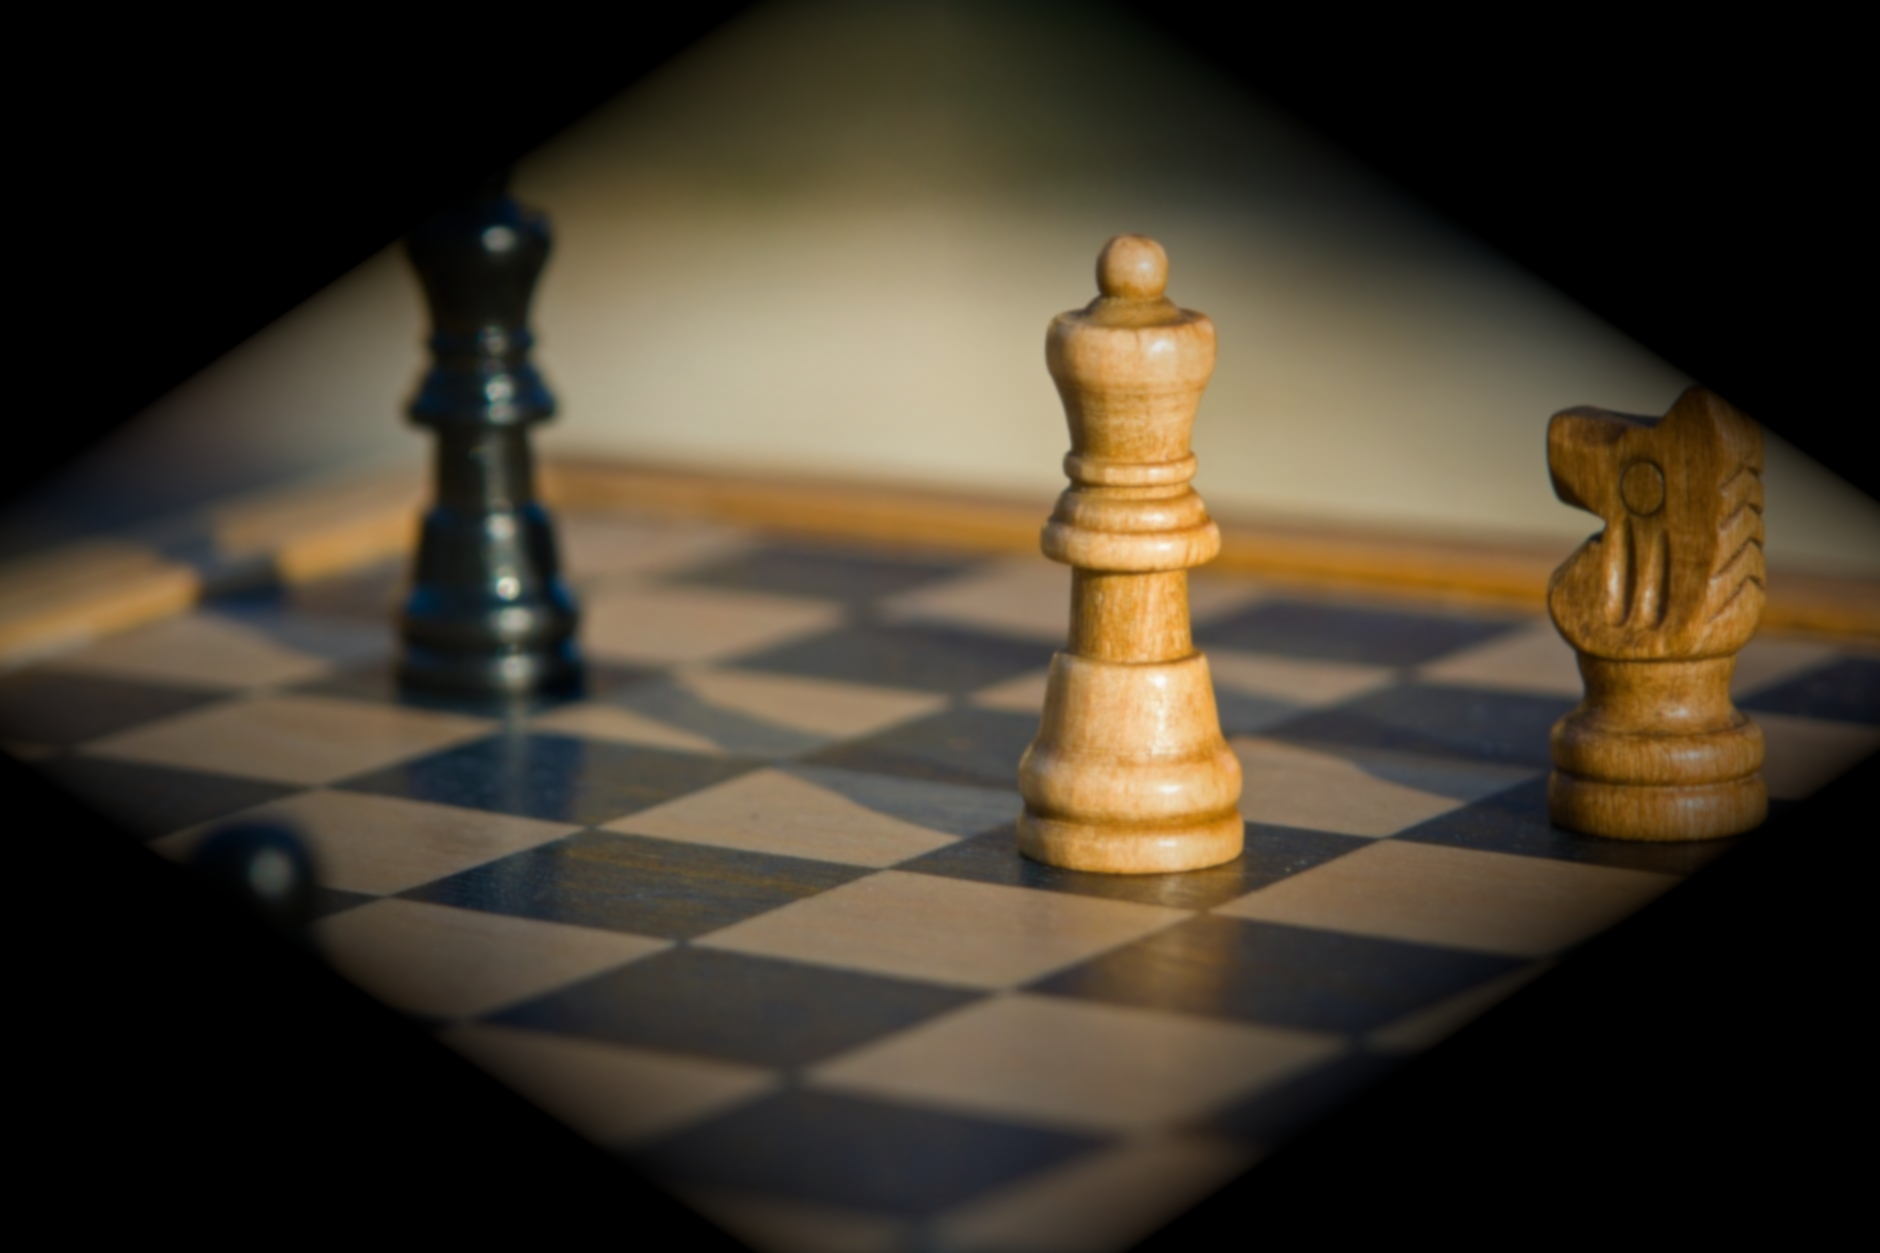
\includegraphics[height=7cm, width=12cm]{Filters/Chess-Vignette.jpeg}
\end{figure}

\subsection*{\flushleft{Output: Filter - Lighting}}
\begin{figure}[h]
\centering
\caption{Filter: Lighting}
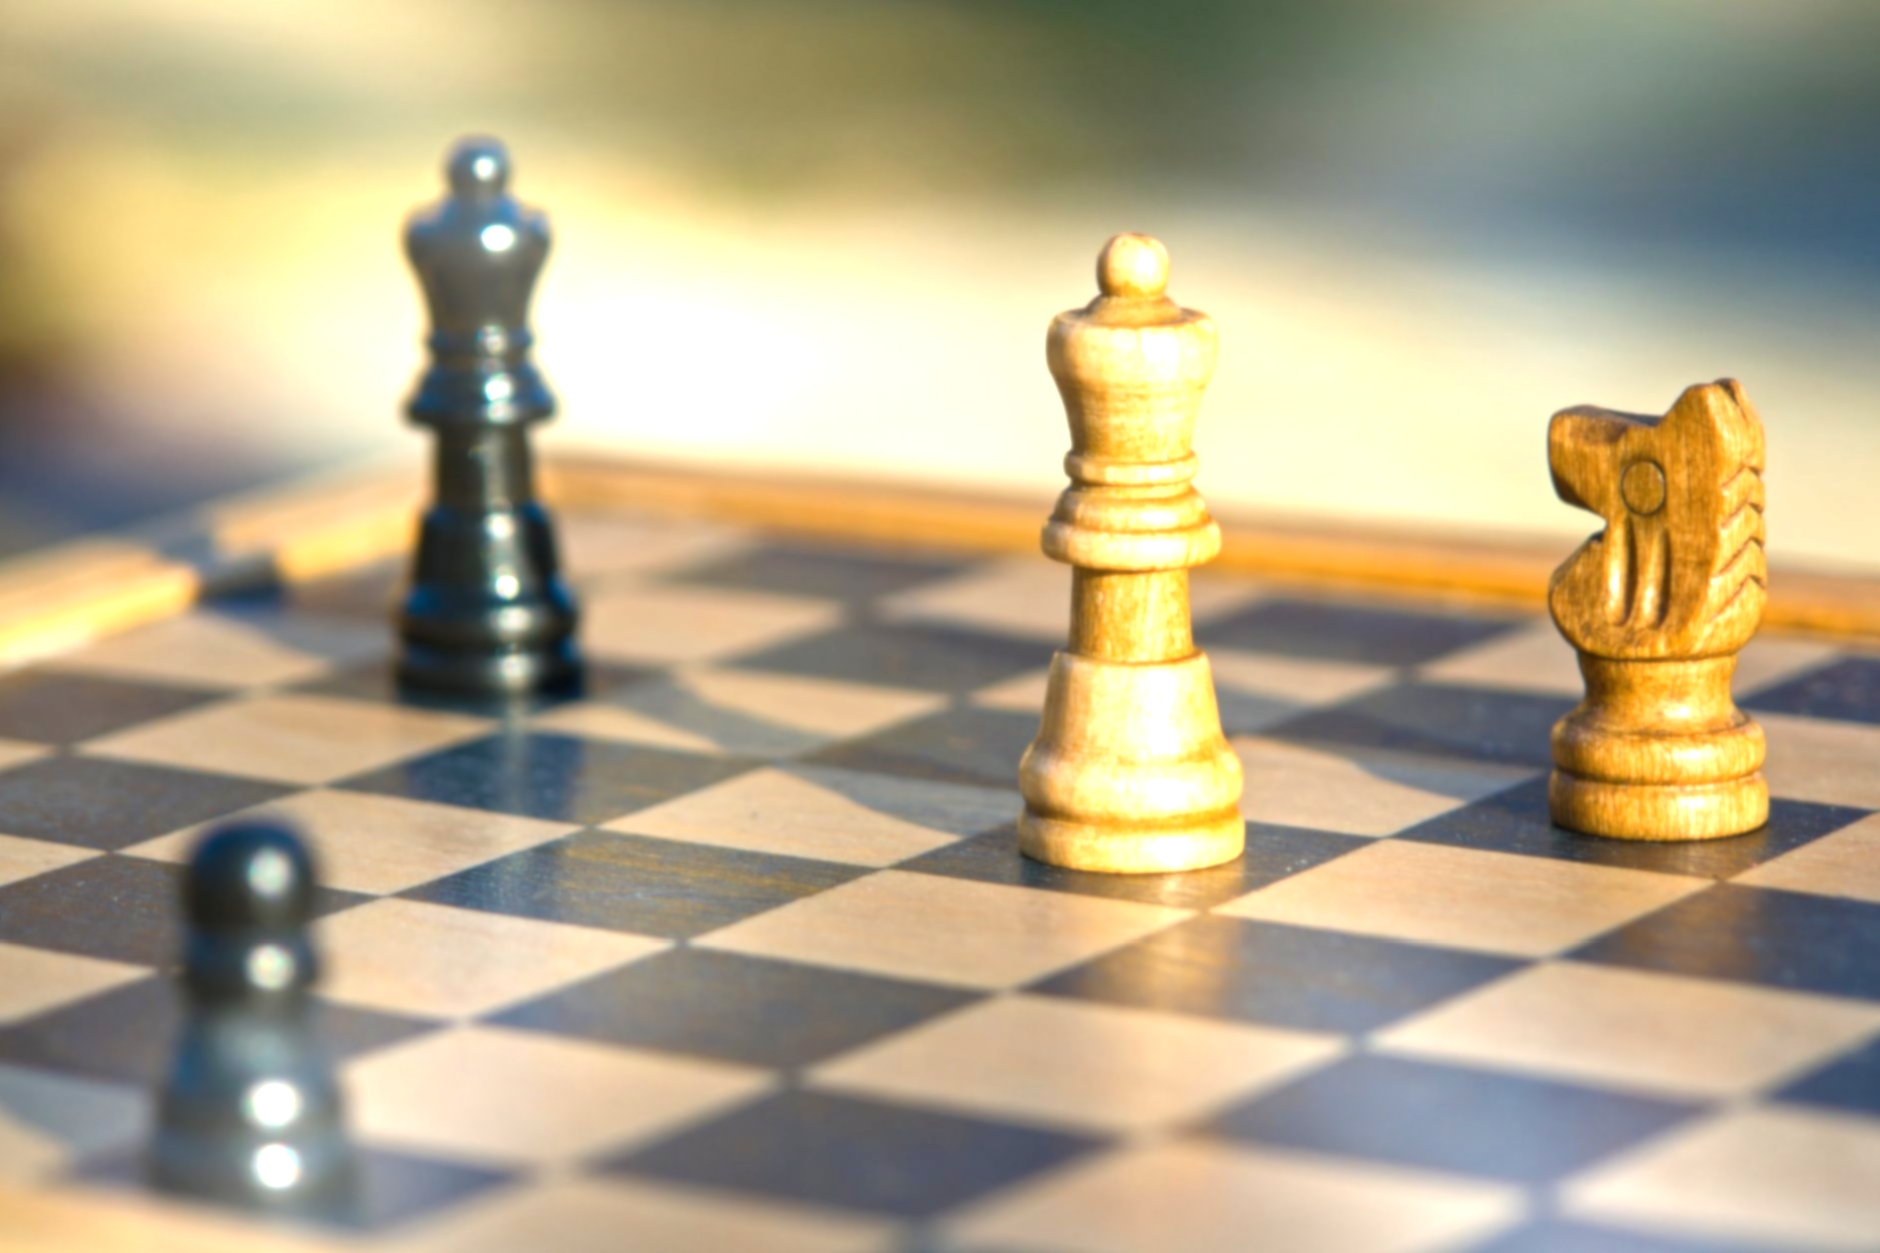
\includegraphics[height=7cm, width=12cm]{Filters/Chess-Lighting.jpeg}
\end{figure}

\newpage
\subsection*{\flushleft{Output: Filter - Gaussian Blur}}
\begin{figure}[h]
\centering
\caption{Filter: Gaussian Blur}
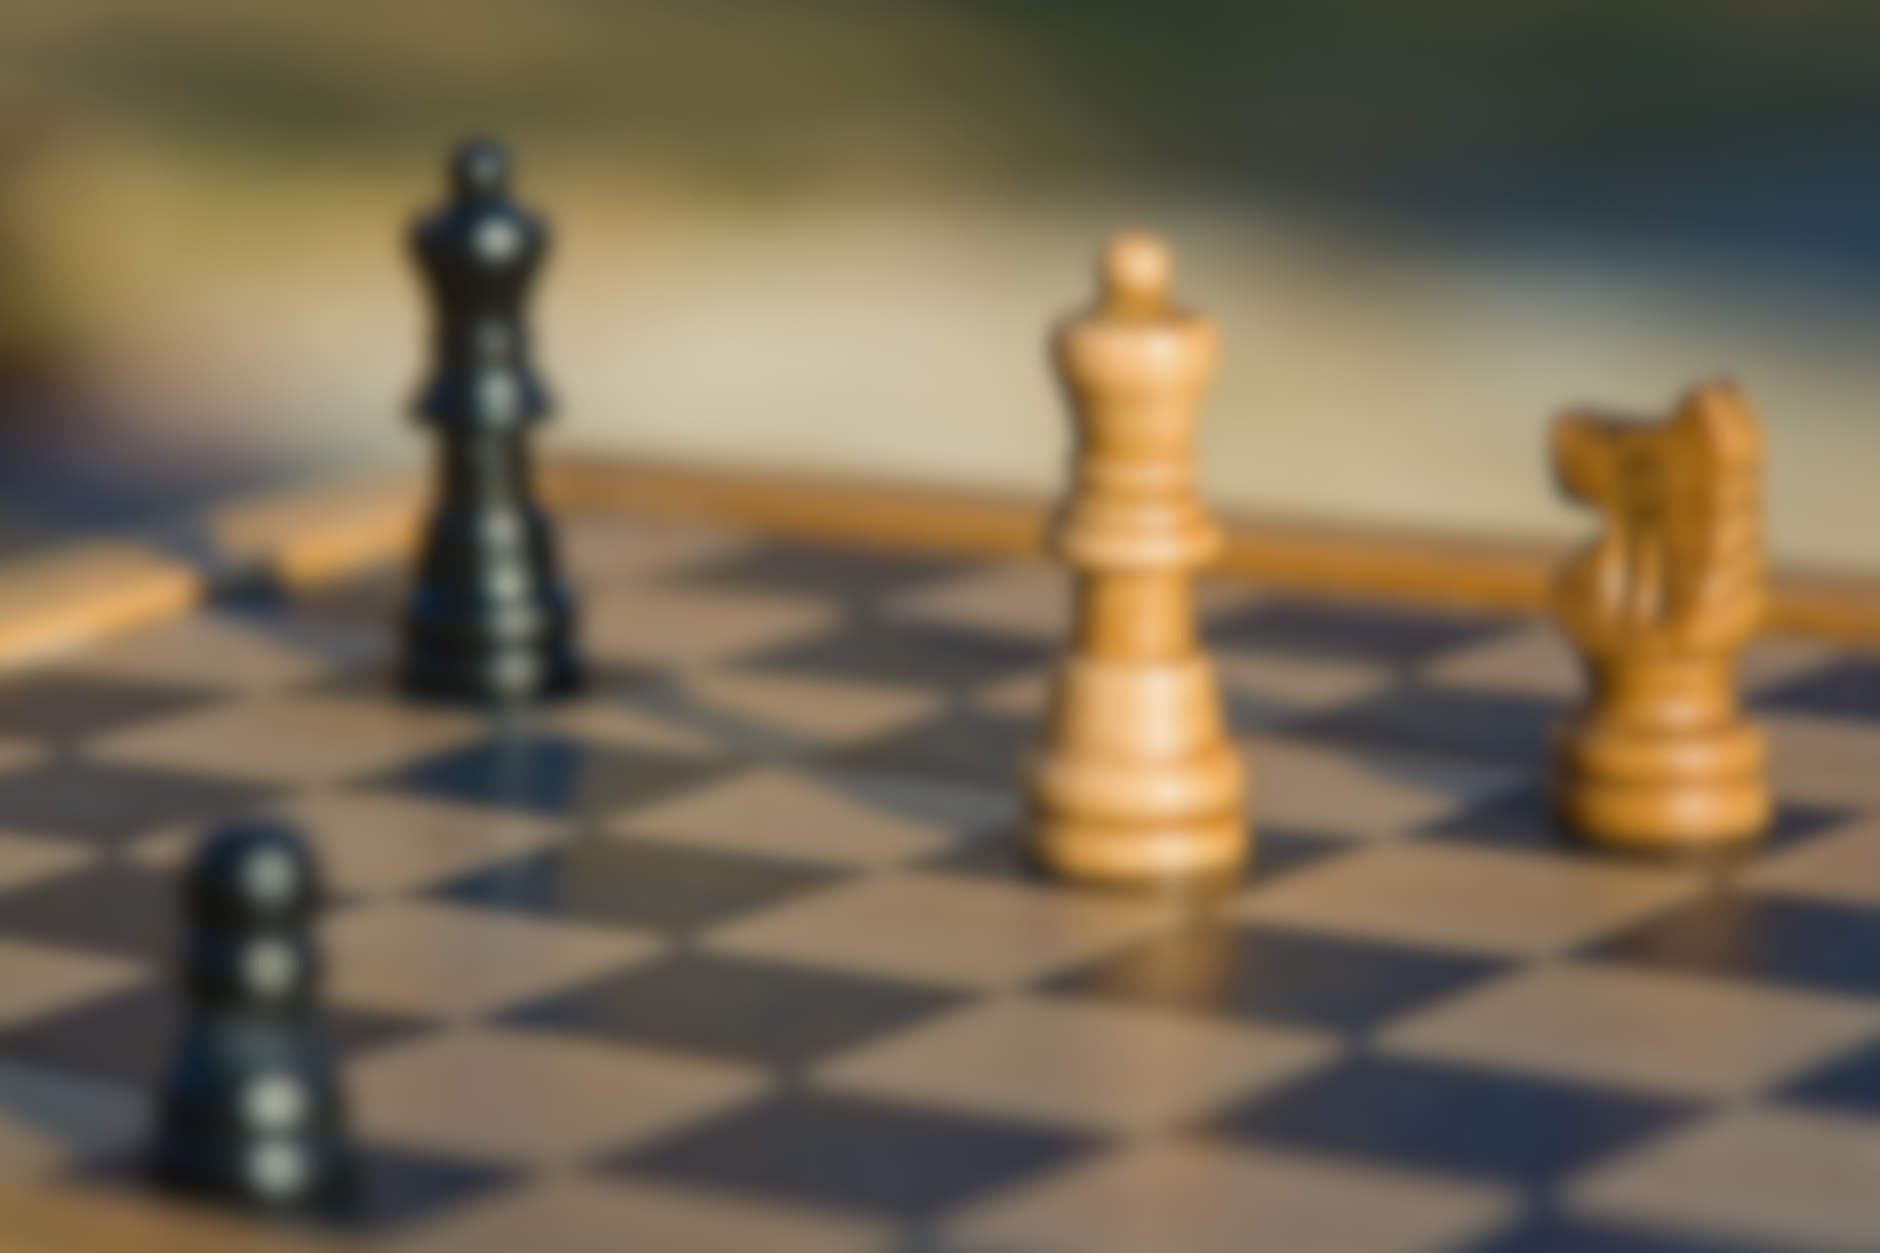
\includegraphics[height=7cm, width=12cm]{Filters/Chess-GaussianBlur.jpeg}
\end{figure}

\subsection*{\flushleft{Output: Filter - Edge Detect}}
\begin{figure}[h]
\centering
\caption{Filter: Edge Detect}
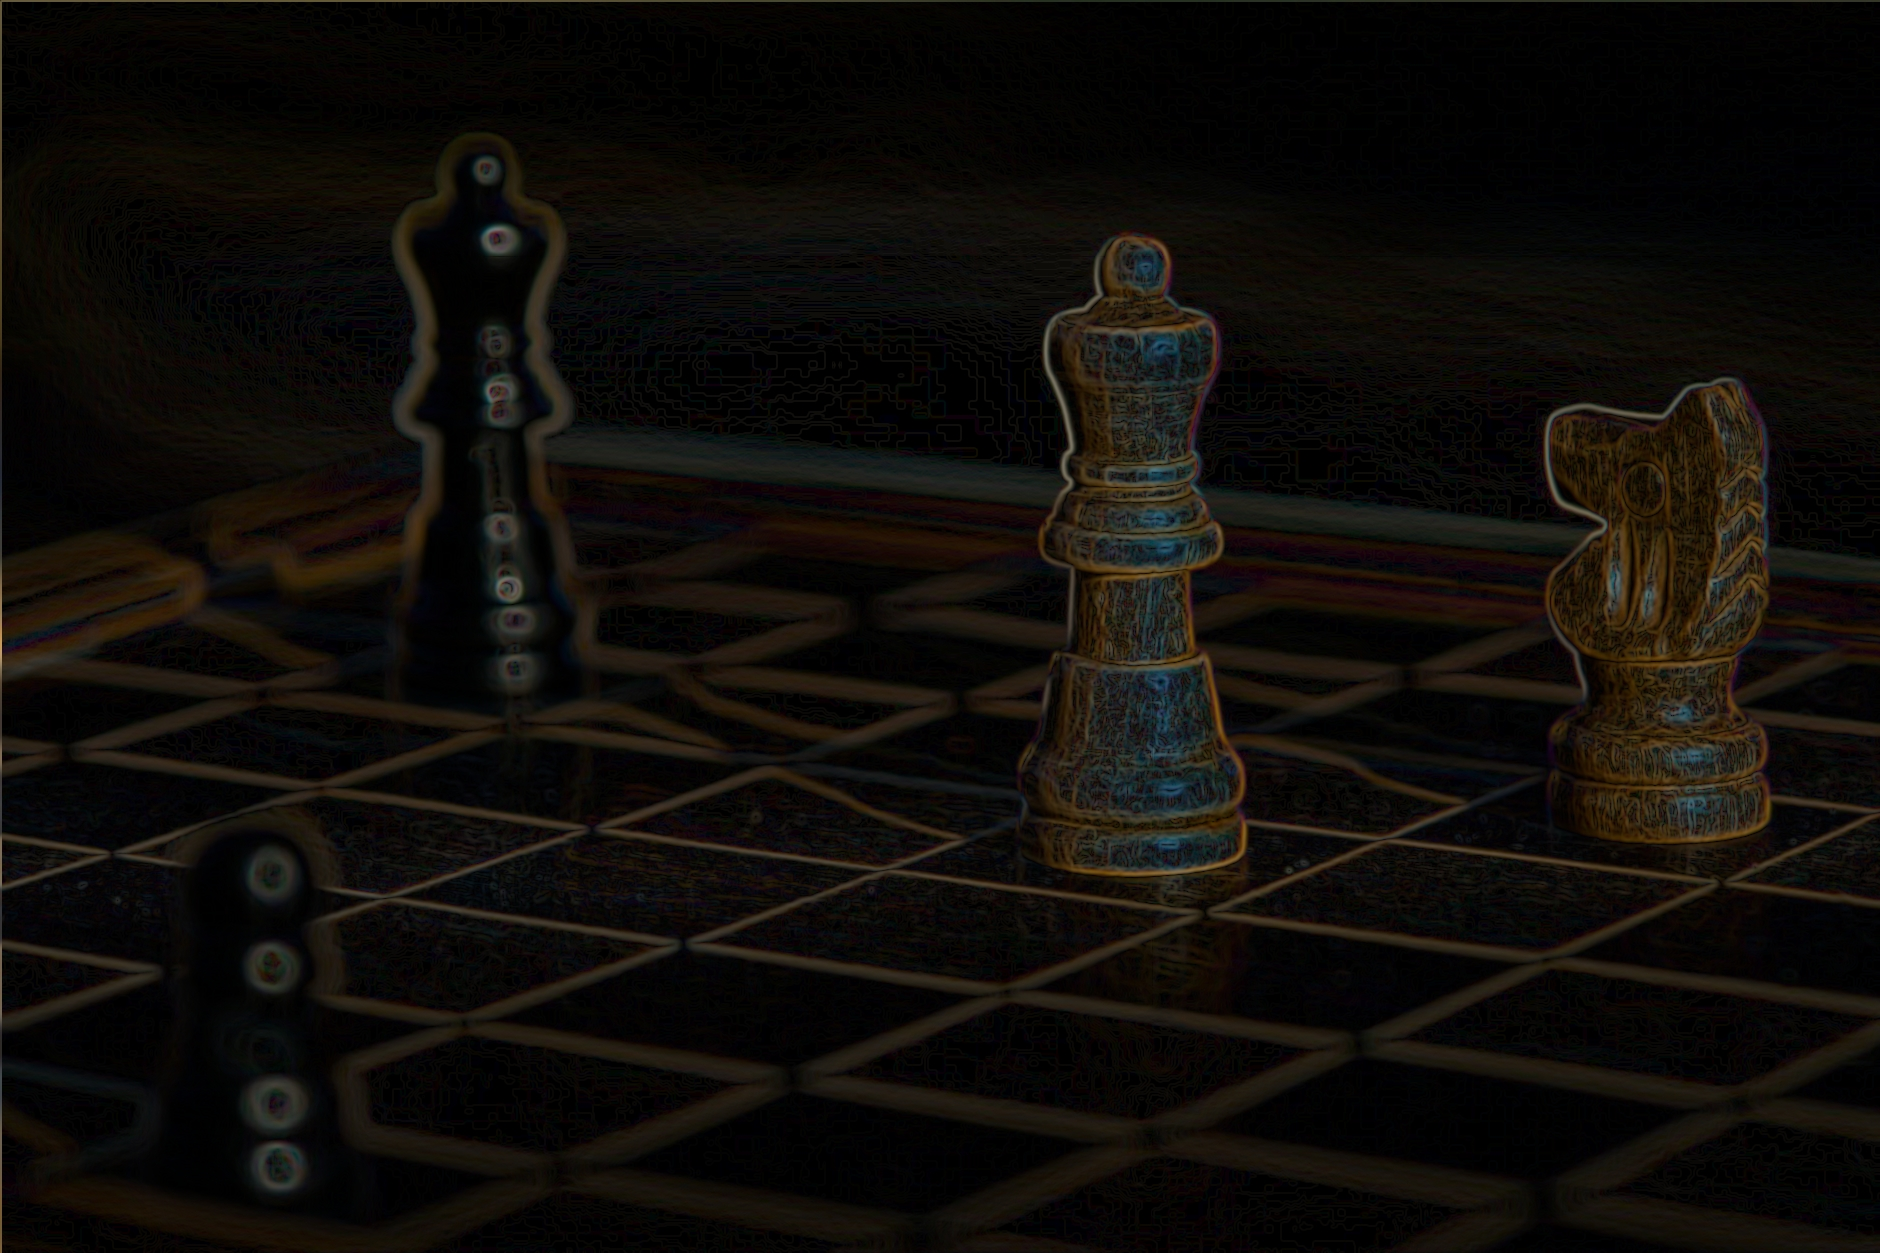
\includegraphics[height=7cm, width=12cm]{Filters/Chess-EdgeDetect.jpeg}
\end{figure}

\newpage
\subsection*{\flushleft{Output: Filter - Cartoon}}
\begin{figure}[h]
\centering
\caption{Filter: Cartoon}
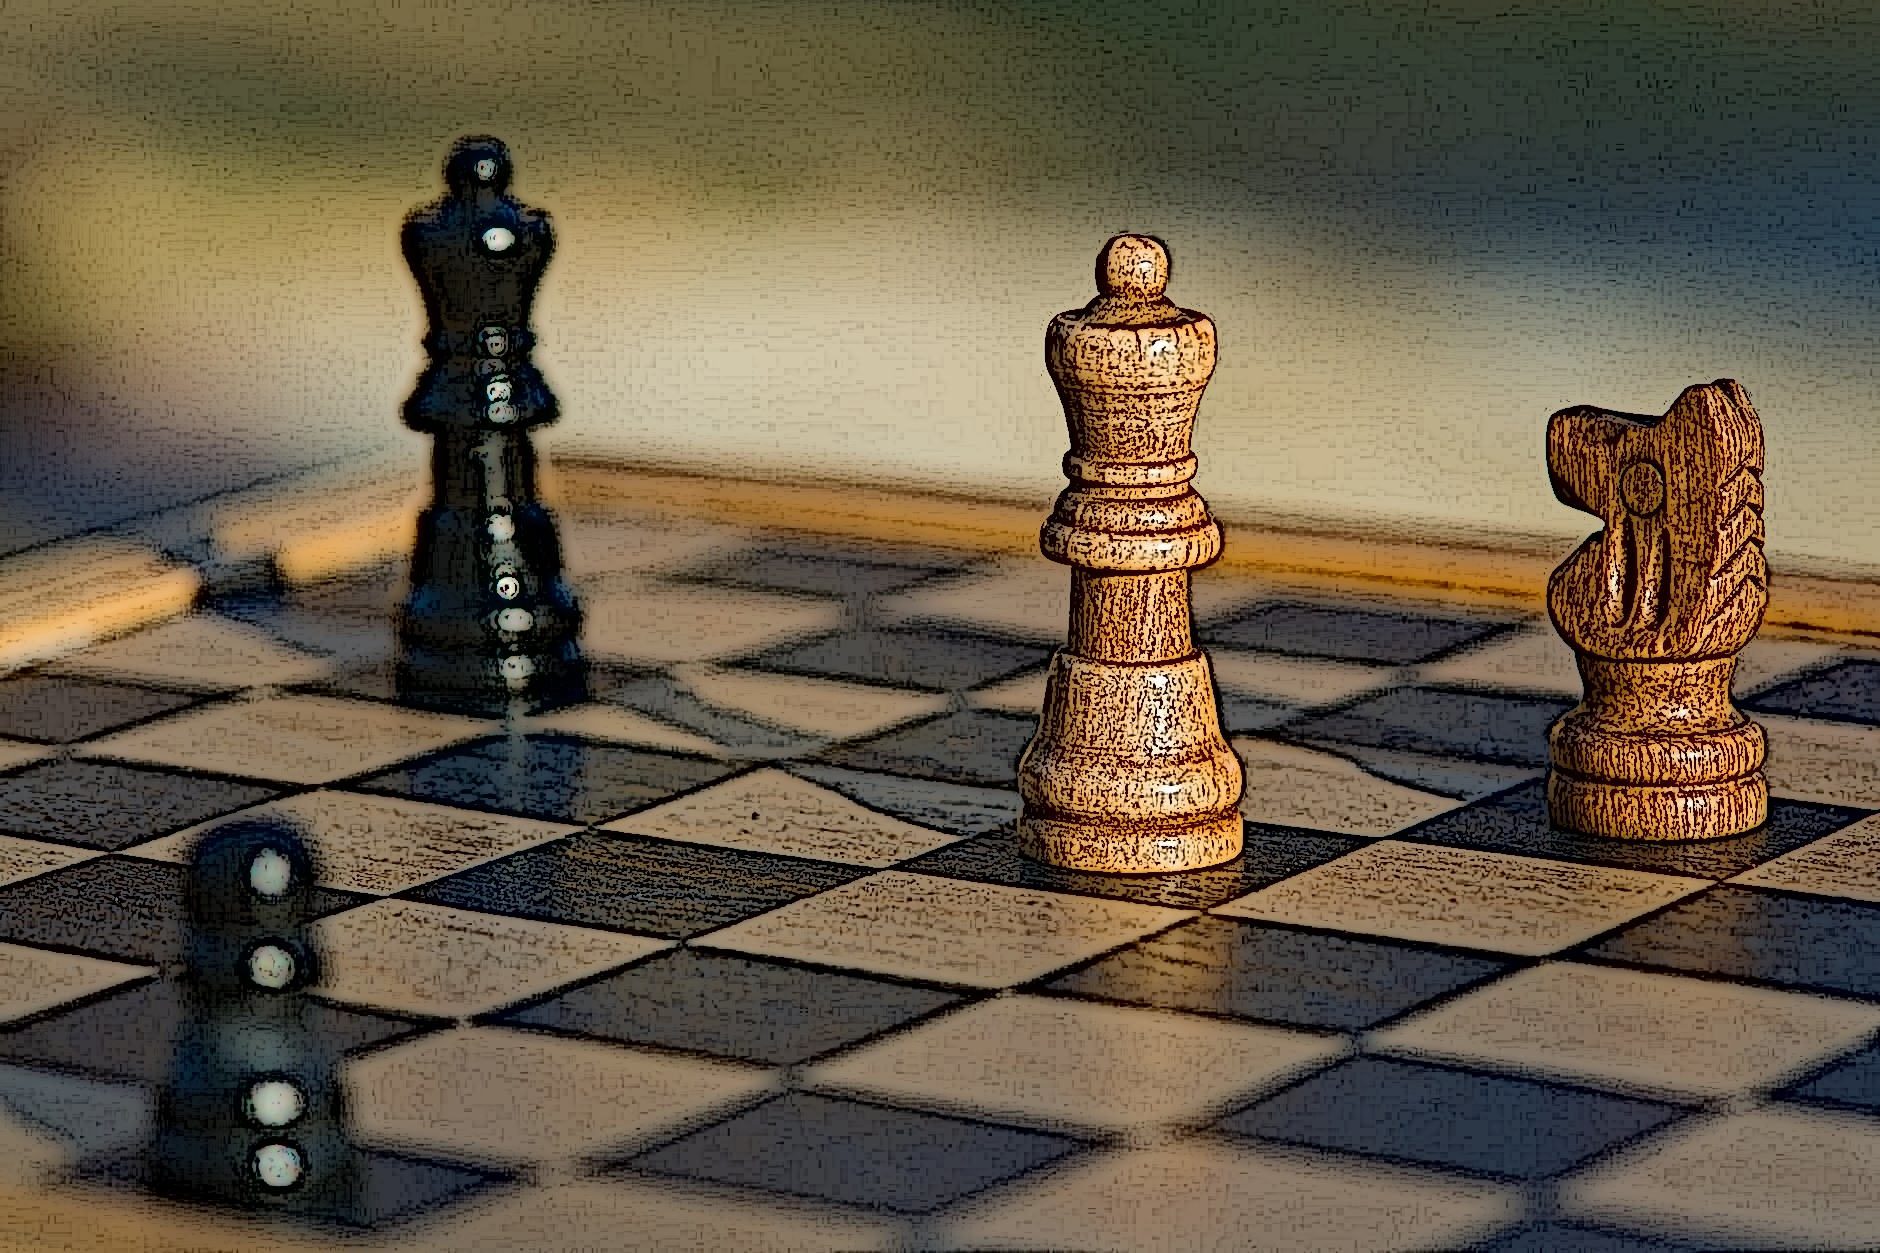
\includegraphics[height=7cm, width=12cm]{Filters/Chess-Cartoon.jpeg}
\end{figure}

\subsection*{\flushleft{Output: Noise - RGB Noise}}
\begin{figure}[h]
\centering
\caption{Noise - RGB Noise}
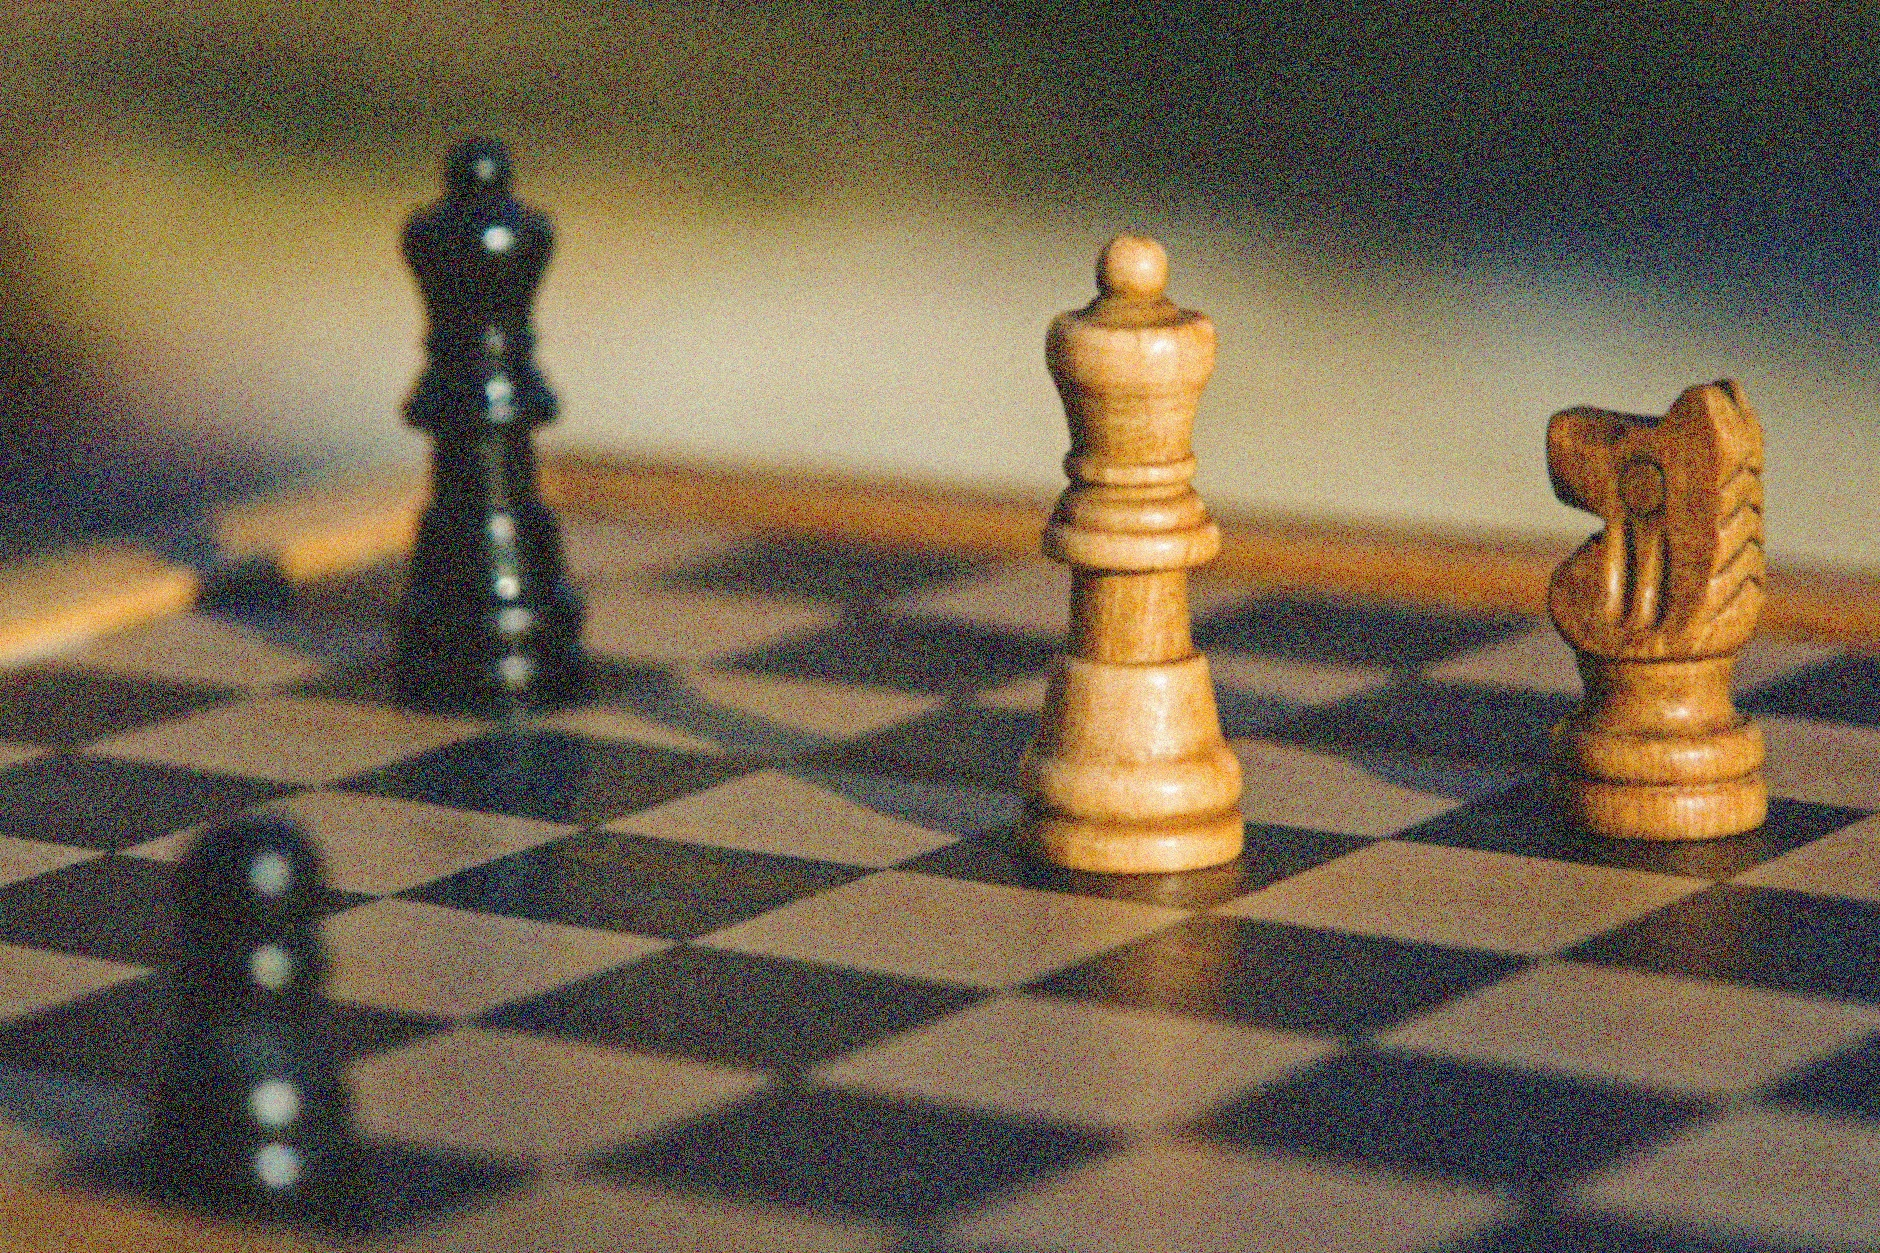
\includegraphics[height=7cm, width=12cm]{Noise/Chess-RGBNoise.jpeg}
\end{figure}

\newpage
\subsection*{\flushleft{Output: Noise - CIE Noise}}
\begin{figure}[h]
\centering
\caption{Noise - CIE Noise}
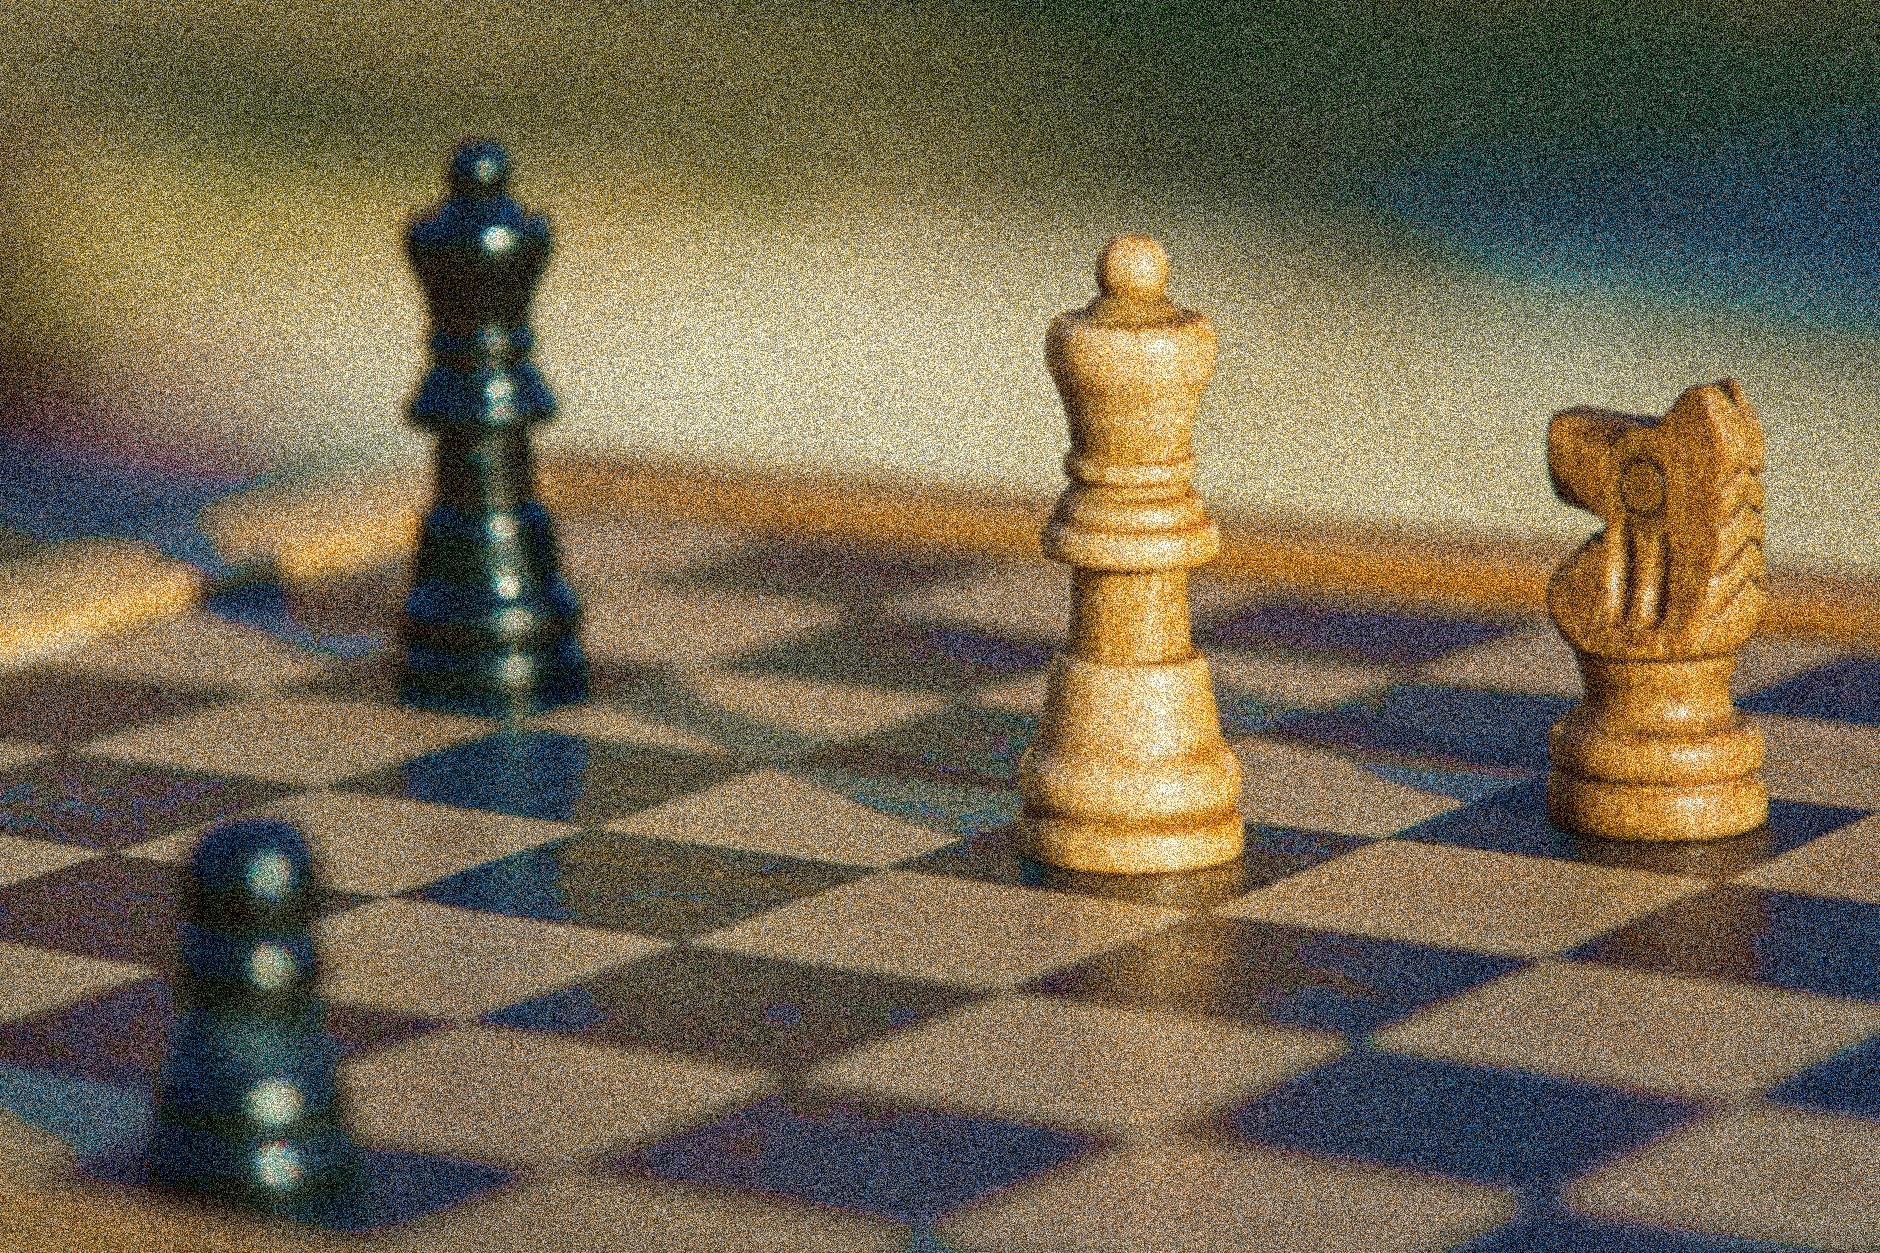
\includegraphics[height=7cm, width=12cm]{Noise/Chess-CIENoise.jpeg}
\end{figure}

\subsection*{\flushleft{Output: Noise - Hurl Noise}}
\begin{figure}[h]
\centering
\caption{Noise - Hurl Noise}
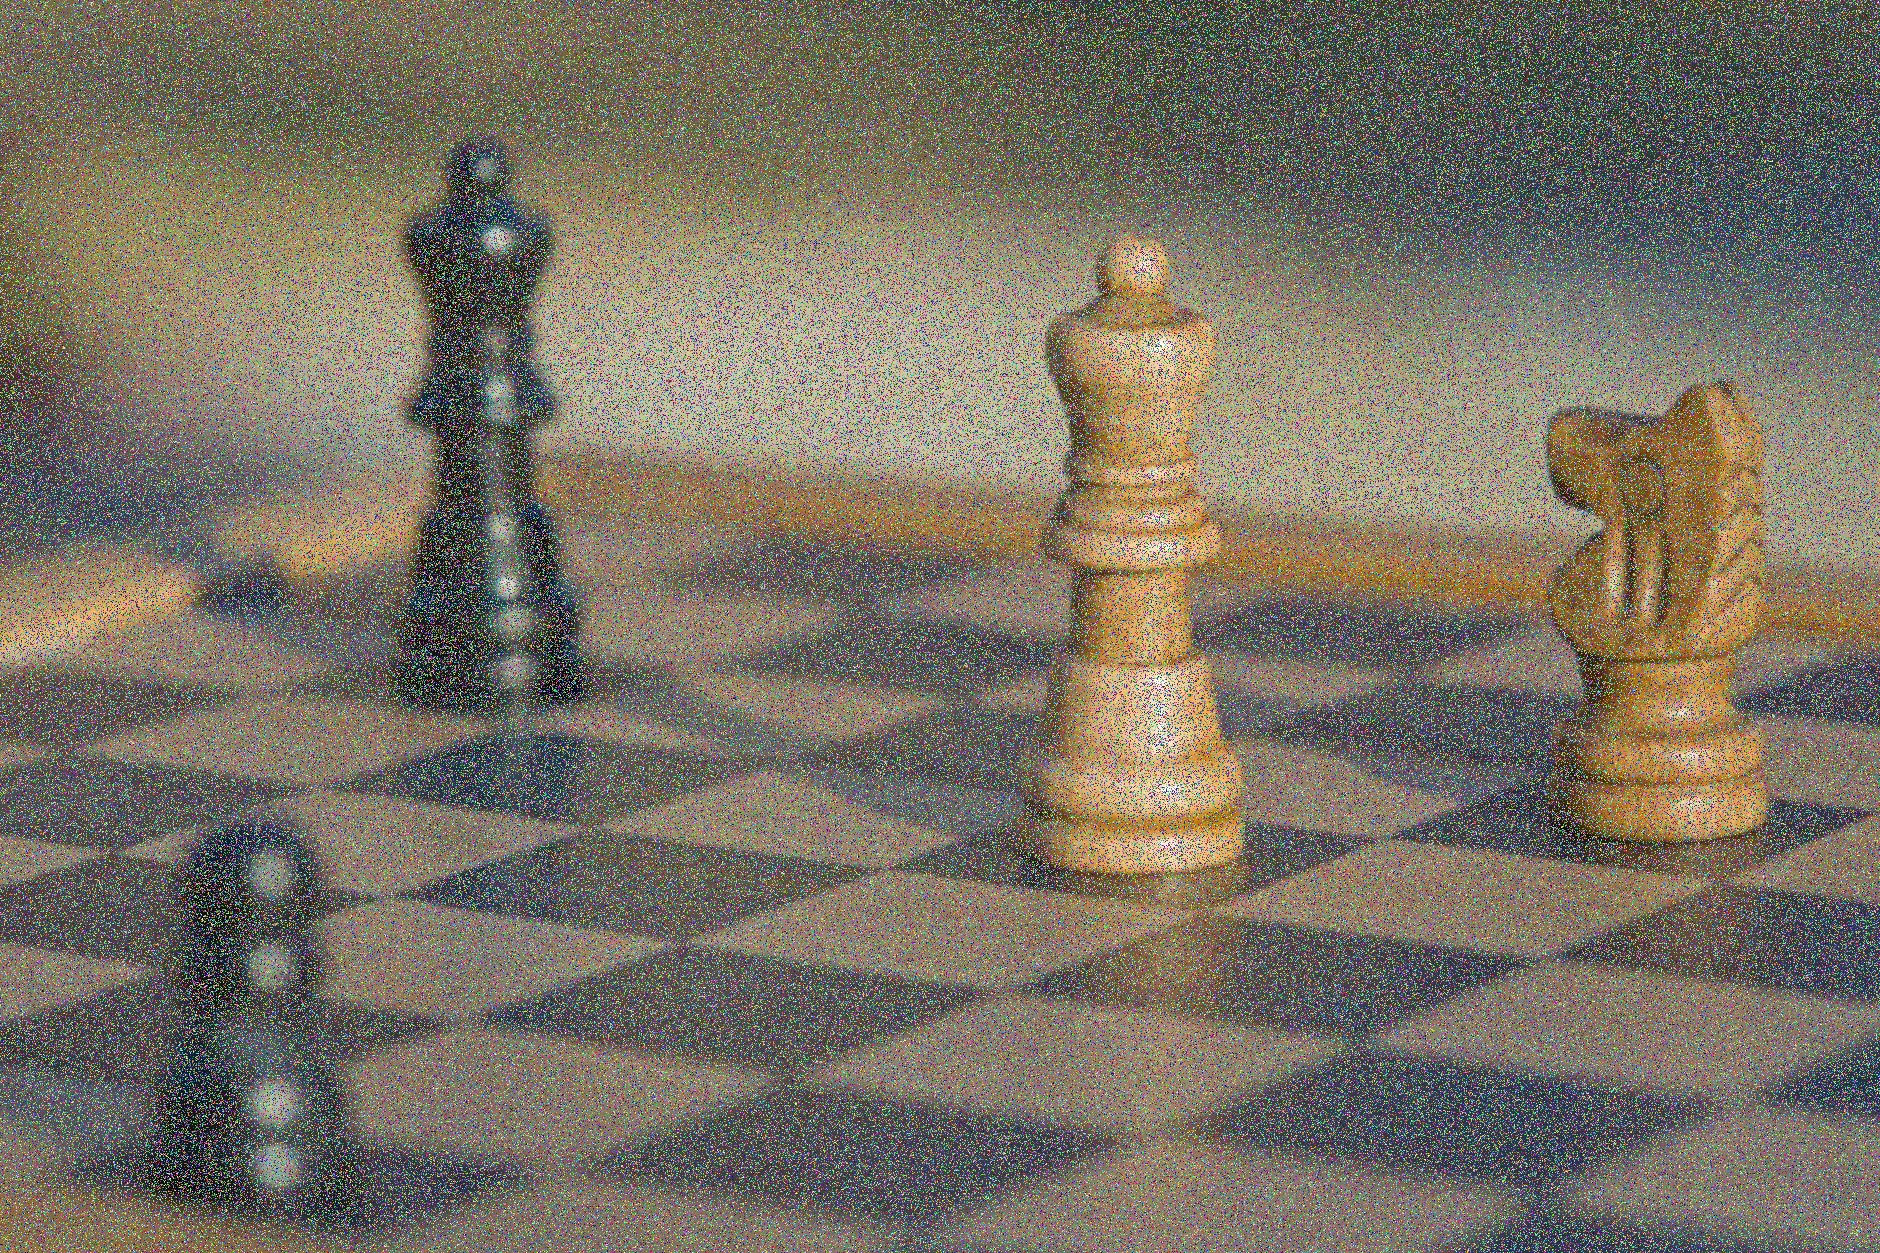
\includegraphics[height=7cm, width=12cm]{Noise/Chess-HurlNoise.jpeg}
\end{figure}


%Input
\newpage
\subsection*{\flushleft{Input: Base Image}}
\begin{figure}[h]
\centering
\caption{Base Image.}
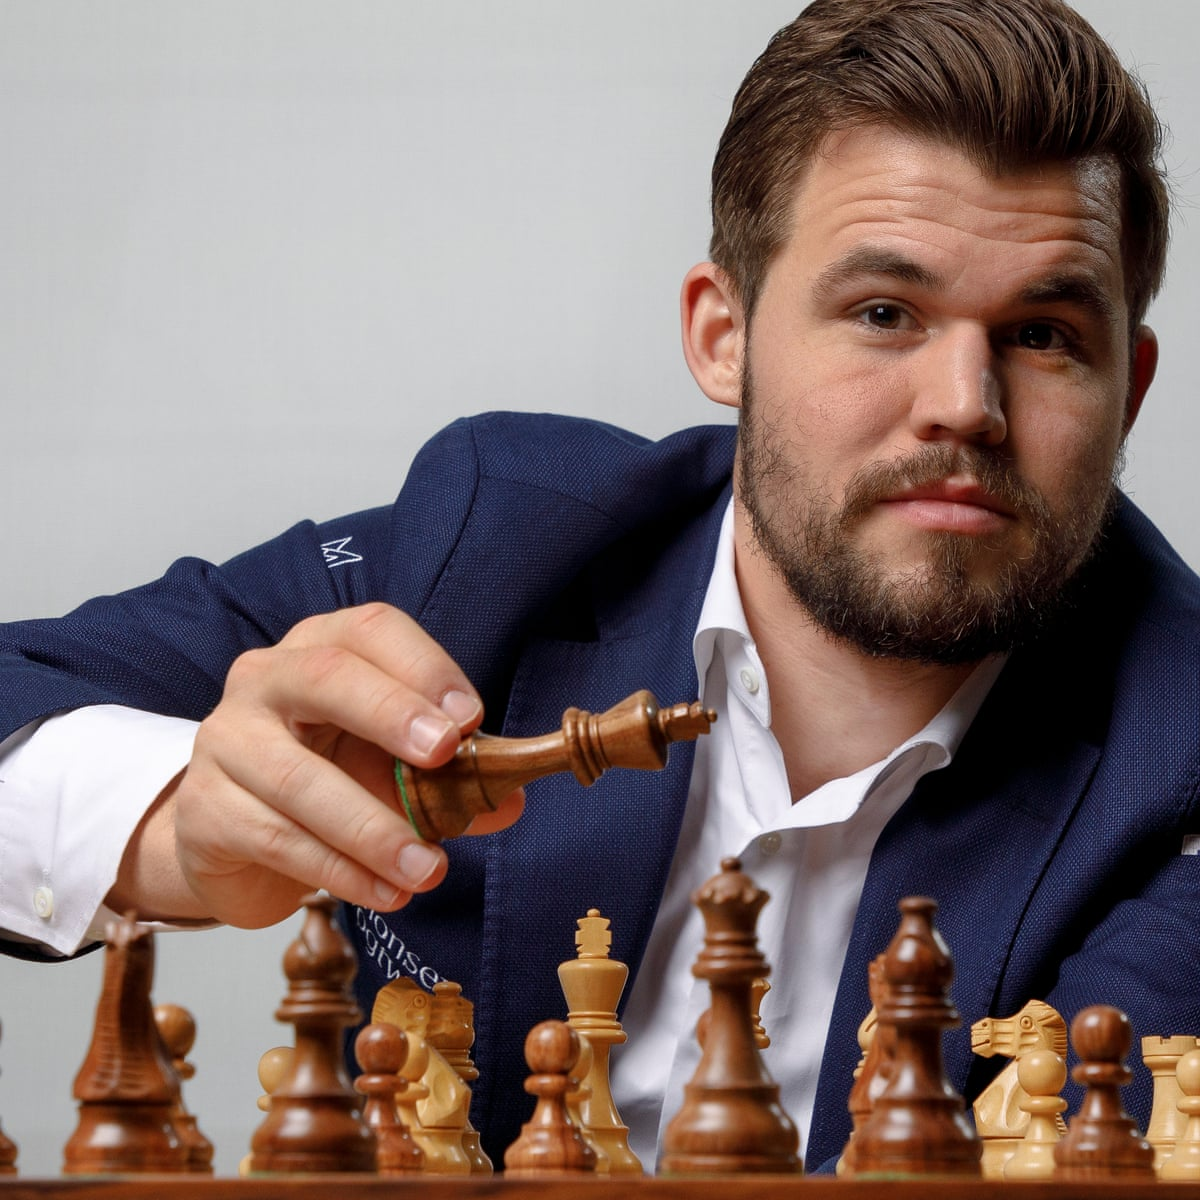
\includegraphics[height=7cm, width=7cm]{Magnus.jpg}
\end{figure}


%Output
\subsection*{\flushleft{Output: Layer Mask}}
\begin{figure}[h]
\centering
\caption{Layer Mask.}
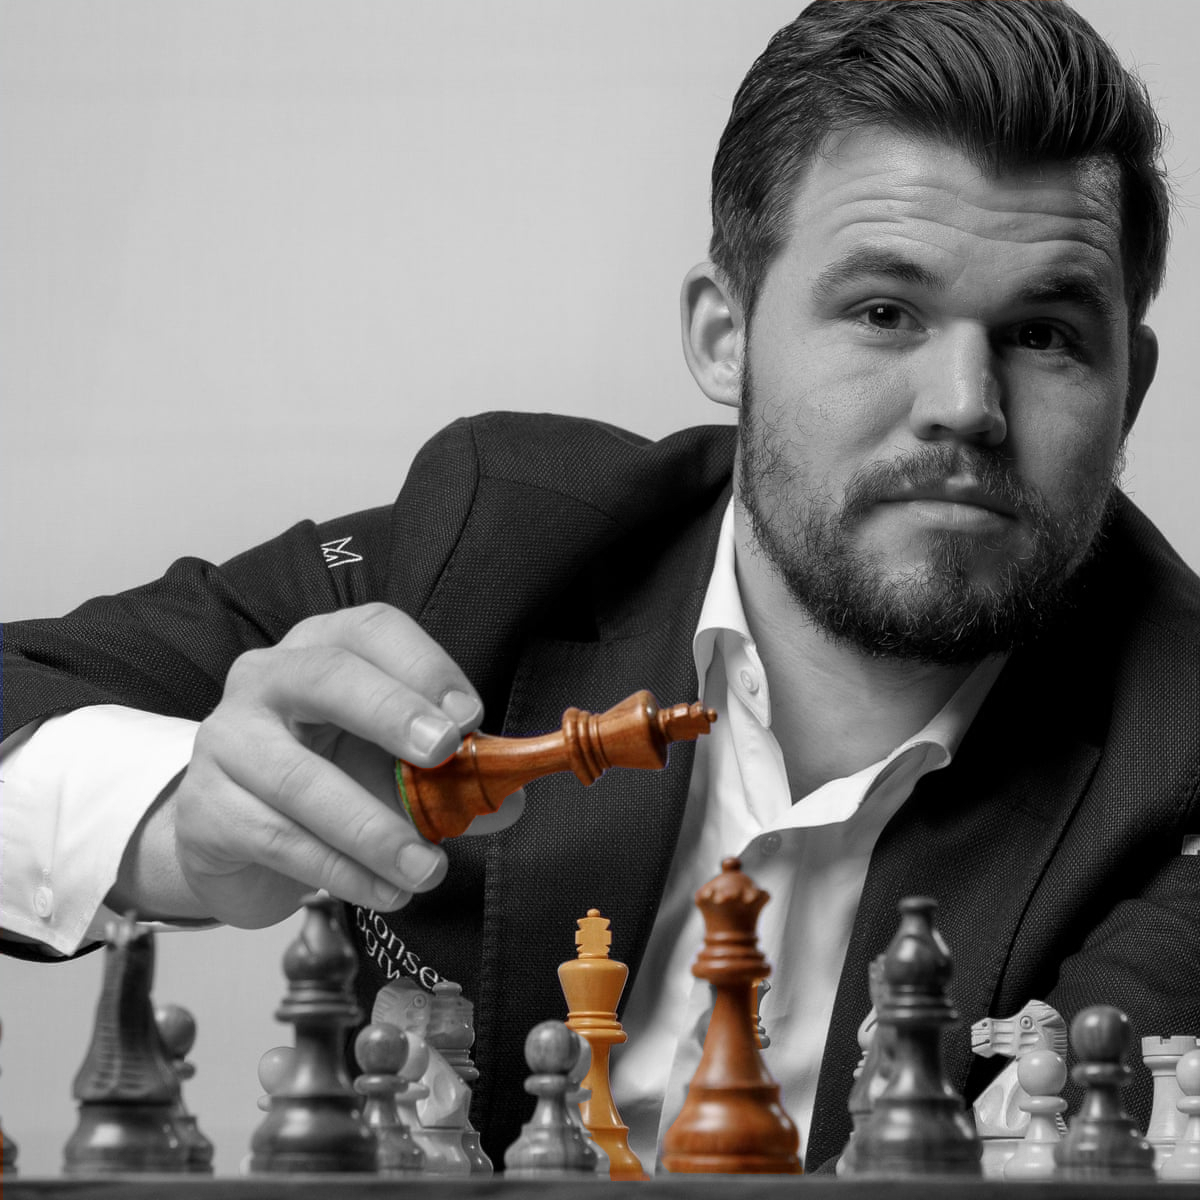
\includegraphics[height=7cm, width=7cm]{Magnus-LayerMask.jpg}
\end{figure}


%Input
\newpage
\subsection*{\flushleft{Input: GIF Image - First}}
\begin{figure}[h]
\centering
\caption{GIF Image - First.}
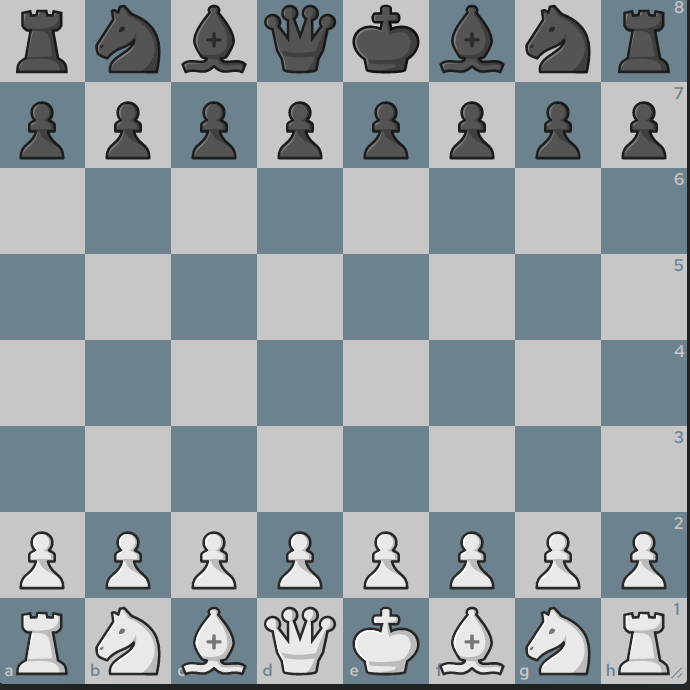
\includegraphics[height=7cm, width=7cm]{GIFImages/0.png}
\end{figure}

\subsection*{\flushleft{Input: GIF Image - Last}}
\begin{figure}[h]
\centering
\caption{GIF Image - Last.}
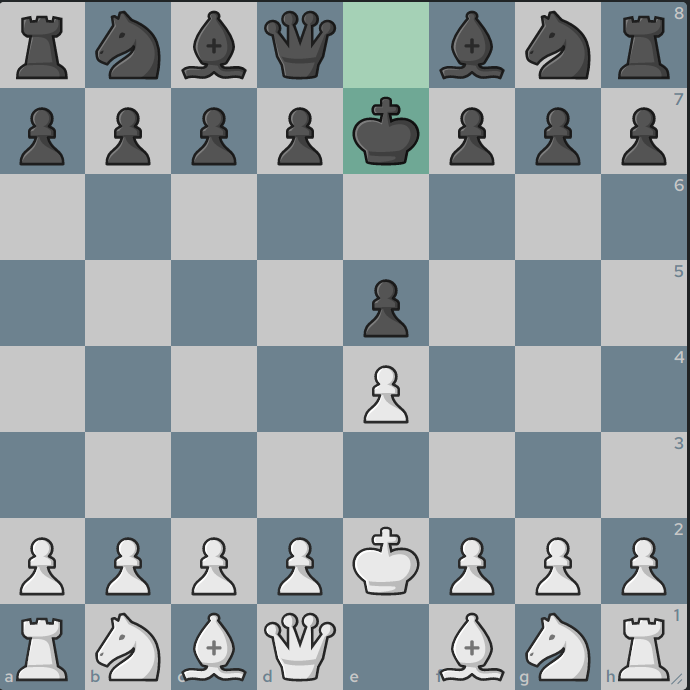
\includegraphics[height=7cm, width=7cm]{GIFImages/12.png}
\end{figure}



%Learning Outcome
\newpage
\subsection*{\flushleft{Learning Outcome:}}
\begin{itemize}
\item I learnt how to use the basic tools of \textbf{GIMP} like the \textbf{Paintbrush, Free Select, Rectangular Select, Eraser, Fill} etc.
\item I understood how to \textbf{apply filters} to an image using GIMP.
\item I learnt how to \textbf{apply noise} to an image using GIMP.
\item I understood how to use \textbf{layer masks} to highlight specific areas of an image.
\item I learnt how to create a \textbf{GIF Image} from a set of static images using GIMP.
\item I understood how to control the \textbf{playback speed} of each image in the GIF.
\item I learnt how to export the edited images/GIF from the GIMP editor to my computer.
\item I learnt about different filters like \textbf{Lighting, Gaussian Blur, Vignette} etc.
\item I also learnt about different types of noise like \textbf{RGB Noise, CIE Noise, Hurl Noise} etc.
\item I learnt how to convert images to \textbf{grayscale} in GIMP.
\end{itemize}


\end{document}